\documentclass[tikz]{standalone}
\usetikzlibrary{backgrounds}	% Frame around tikzpicture
\usetikzlibrary{positioning}
\usepackage[none]{hyphenat}		% Prevent hyphenation

\newcommand{\posit}{{\color{red}\textcircled{$+$}}}
\newcommand{\negat}{\textcircled{$-$}}

\newcommand{\xshiftvar}{5mm}
\newcommand{\yshiftvar}{3mm}

\tikzstyle{pid} = [font=\Huge, anchor=north west]
\tikzstyle{heading} = [font=\Large, anchor=north west, yshift=-\yshiftvar]
\tikzstyle{label} = [anchor=north west]
\tikzstyle{field} = [draw=black, anchor=north west, xshift=\xshiftvar]
\tikzstyle{tab} = [draw=black, minimum height=6mm]

\begin{document}
	
	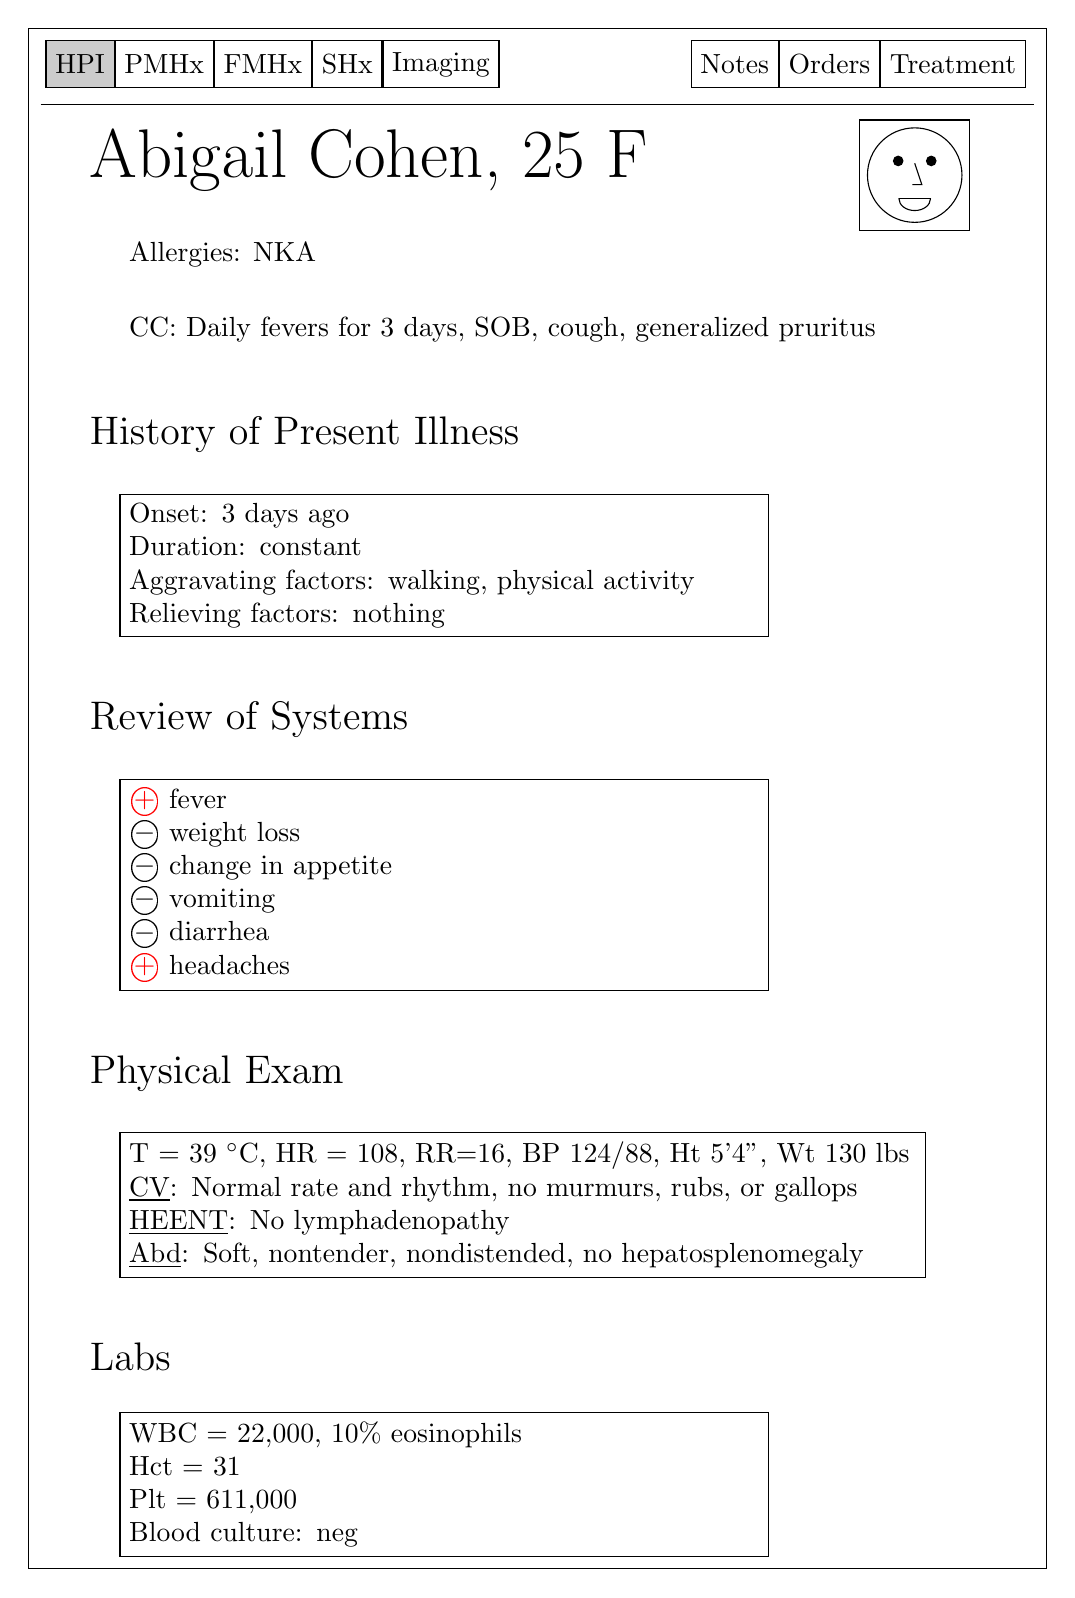
\begin{tikzpicture}[framed, node distance=4mm]

		\node (pid) [pid] {Abigail Cohen, 25 F};

		\draw [] (9.9,-1.4) rectangle (11.3,0);
		\draw [] (10.6,-0.7) circle (6mm);
		\draw [fill=black] (10.39,-0.52) circle (0.6mm);
		\draw [fill=black] (10.81,-0.52) circle (0.6mm);
		\draw [black] (10.6,-0.55) -- (10.69,-0.82) -- (10.57,-0.82);
		\begin{scope}
			\clip (10.38,-1.2) rectangle (10.82,-0.996);
			\draw (10.6,-1) ellipse (0.2 and 0.15);
			\draw (10.4,-1) -- (10.8,-1);
		\end{scope})

		\node (allergy) [below=of pid.south west, label, xshift=\xshiftvar] {Allergies: NKA};

		\node (cc) [below=of allergy.south west, label] {CC: Daily fevers for 3 days, SOB, cough, generalized pruritus};

		\node (hpi_head) [below=of cc.south west, heading, xshift=-\xshiftvar] {History of Present Illness};

		\node (hpi) [below=of hpi_head.south west, field, text width=8cm] {
			Onset: 3 days ago\\
			Duration: constant\\
			Aggravating factors: walking, physical activity\\
			Relieving factors: nothing
		};

		\node (ros_head) [below=of hpi.south west, heading, xshift=-\xshiftvar] {Review of Systems};

		\node (ros) [below=of ros_head.south west, field, text width=8cm] {
			\posit\ fever\\
			\negat\ weight loss\\
			\negat\ change in appetite\\
			\negat\ vomiting\\
			\negat\ diarrhea\\
			\posit\ headaches
		};

		\node (pe_head) [below=of ros.south west, heading, xshift=-\xshiftvar] {Physical Exam};

		\node (pe) [below=of pe_head.south west, field, text width=10cm] {
			T = 39 $^\circ$C, HR = 108, RR=16, BP 124/88, Ht 5'4", Wt 130 lbs\\
			\underline{CV}: Normal rate and rhythm, no murmurs, rubs, or gallops\\
			\underline{HEENT}: No lymphadenopathy\\
			\underline{Abd}: Soft, nontender, nondistended, no hepatosplenomegaly
		};

		\node (labs_head) [below=of pe.south west, heading, xshift=-\xshiftvar] {Labs};

		\node (labs) [below=of labs_head.south west, field, text width=8cm] {WBC = 22,000, 10\% eosinophils\\Hct = 31\\ Plt = 611,000\\Blood culture: neg};


		\draw (-5mm,2mm) -- (\linewidth-\pgflinewidth,2mm);
		\node (hpi_tab) [tab, above=of pid.north west, fill=gray!40] {HPI};
		\node (pmh_tab) [tab, right=of hpi_tab, xshift=-4mm] {PMHx};
		\node (fmh_tab) [tab, right=of pmh_tab, xshift=-4mm] {FMHx};
		\node (sh_tab) [tab, right=of fmh_tab, xshift=-4mm] {SHx};
		\node (img_tab) [tab, right=of sh_tab, xshift=-4mm] {Imaging};
		\node (treat_tab) [tab, above=of pid.north west, xshift=\linewidth-\pgflinewidth-1mm, anchor=south east] {Treatment};
		\node (orders_tab) [tab, left=of treat_tab, xshift=4mm] {Orders};
		\node (notes_tab) [tab, left=of orders_tab, xshift=4mm] {Notes};

	\end{tikzpicture}
		
\end{document}